\section{Design}
\subsection{High level system design}
\begin{figure}[h]
    \centering
    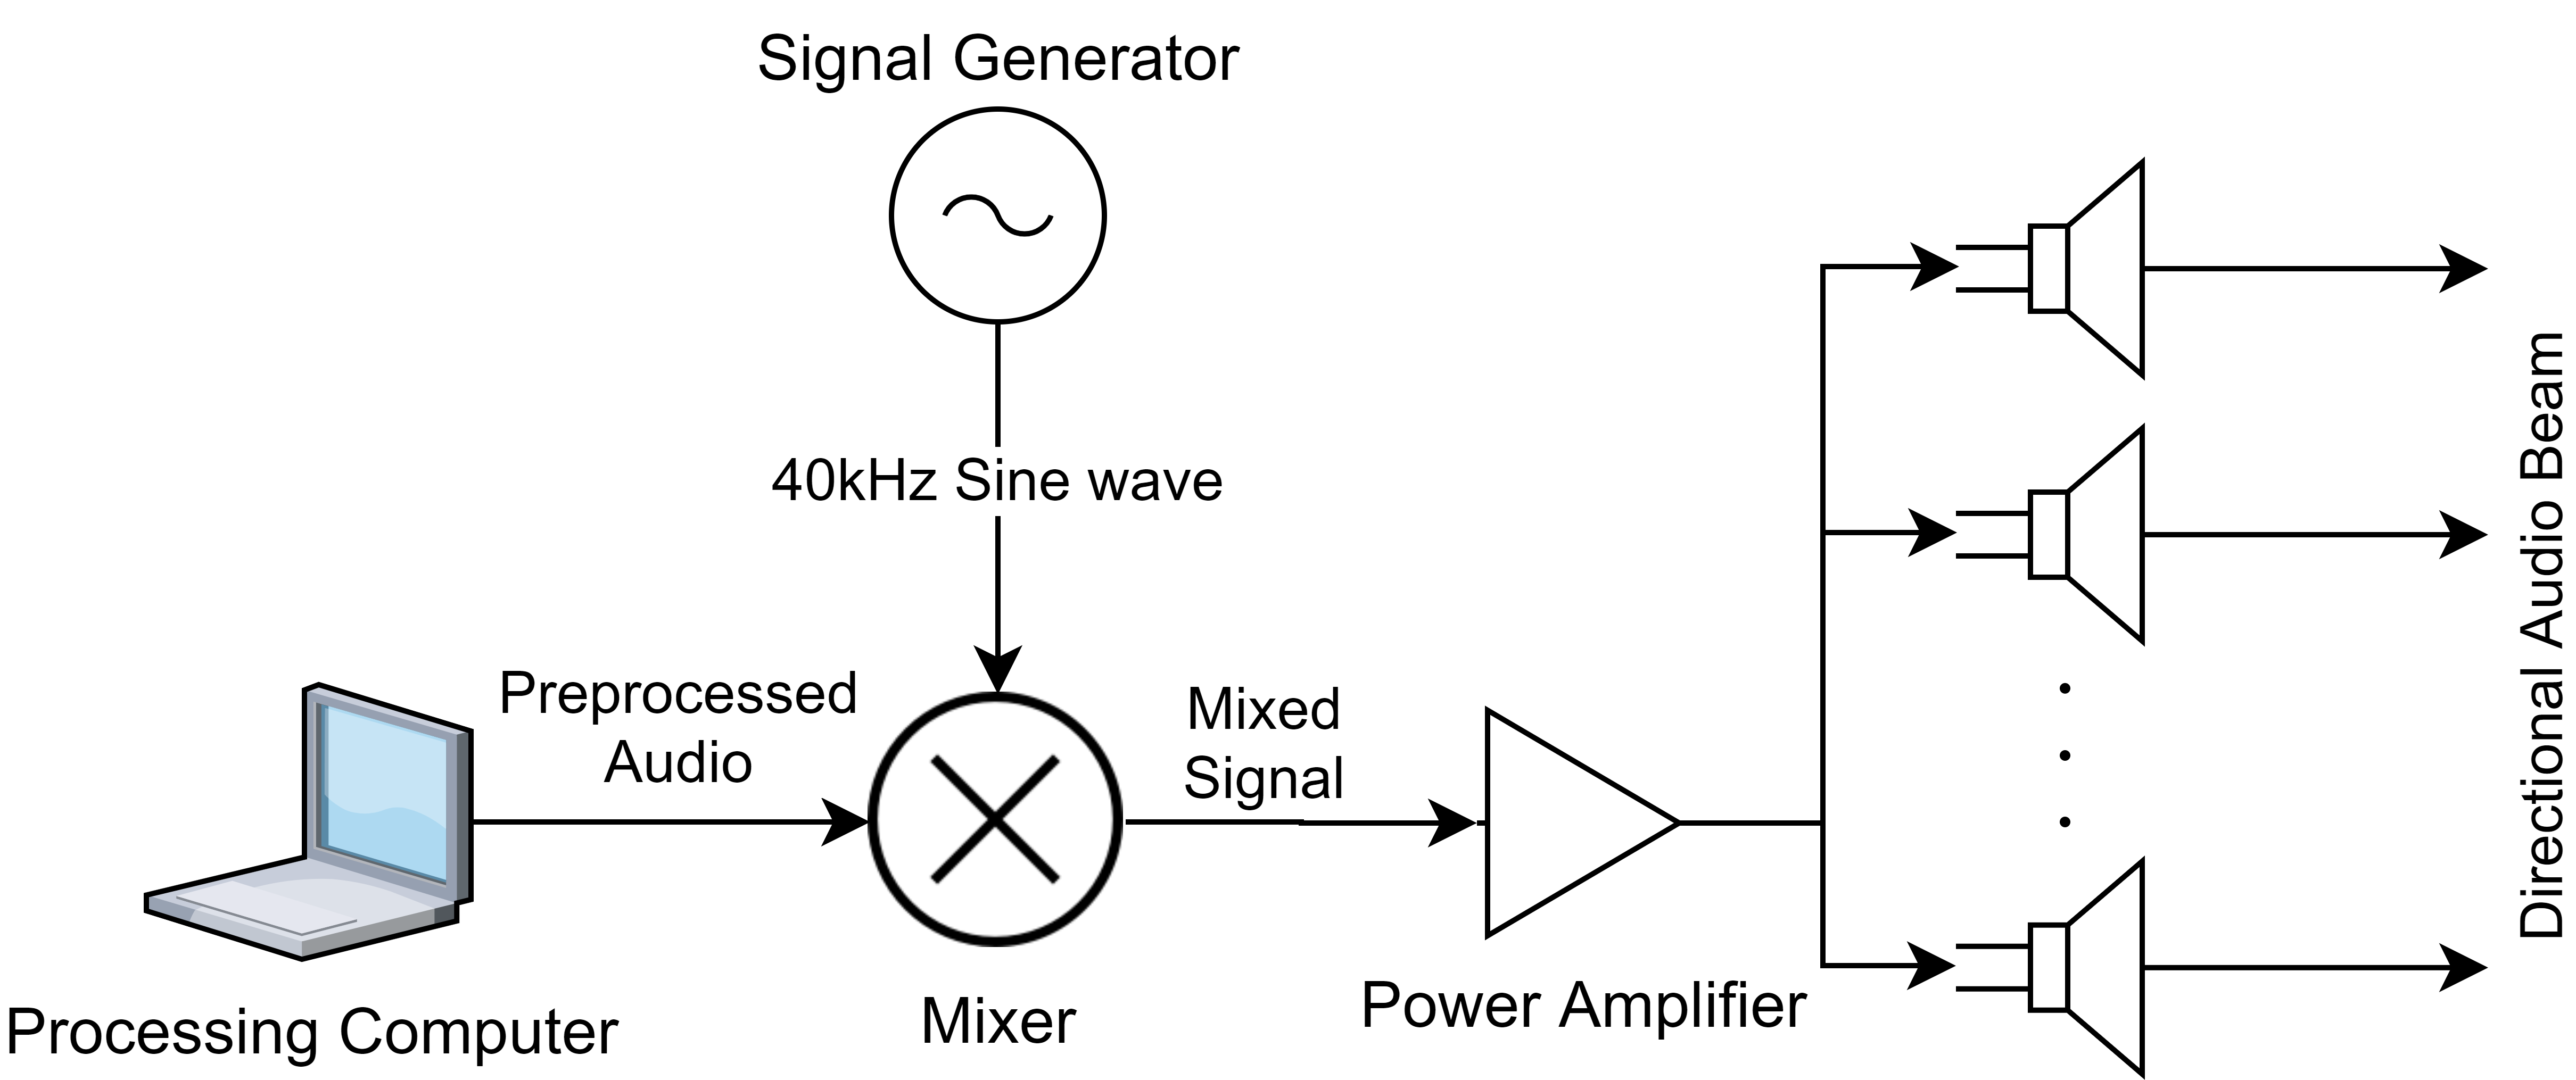
\includegraphics[width=\textwidth]{Figures/HighlevelSystemDesign.png}
    \caption{High level system design for the directional audio system}
    \label{fig:highleveldesign}
\end{figure}
\subsection{Pre-processing subsystem design}
\begin{figure}[h]
    \centering
    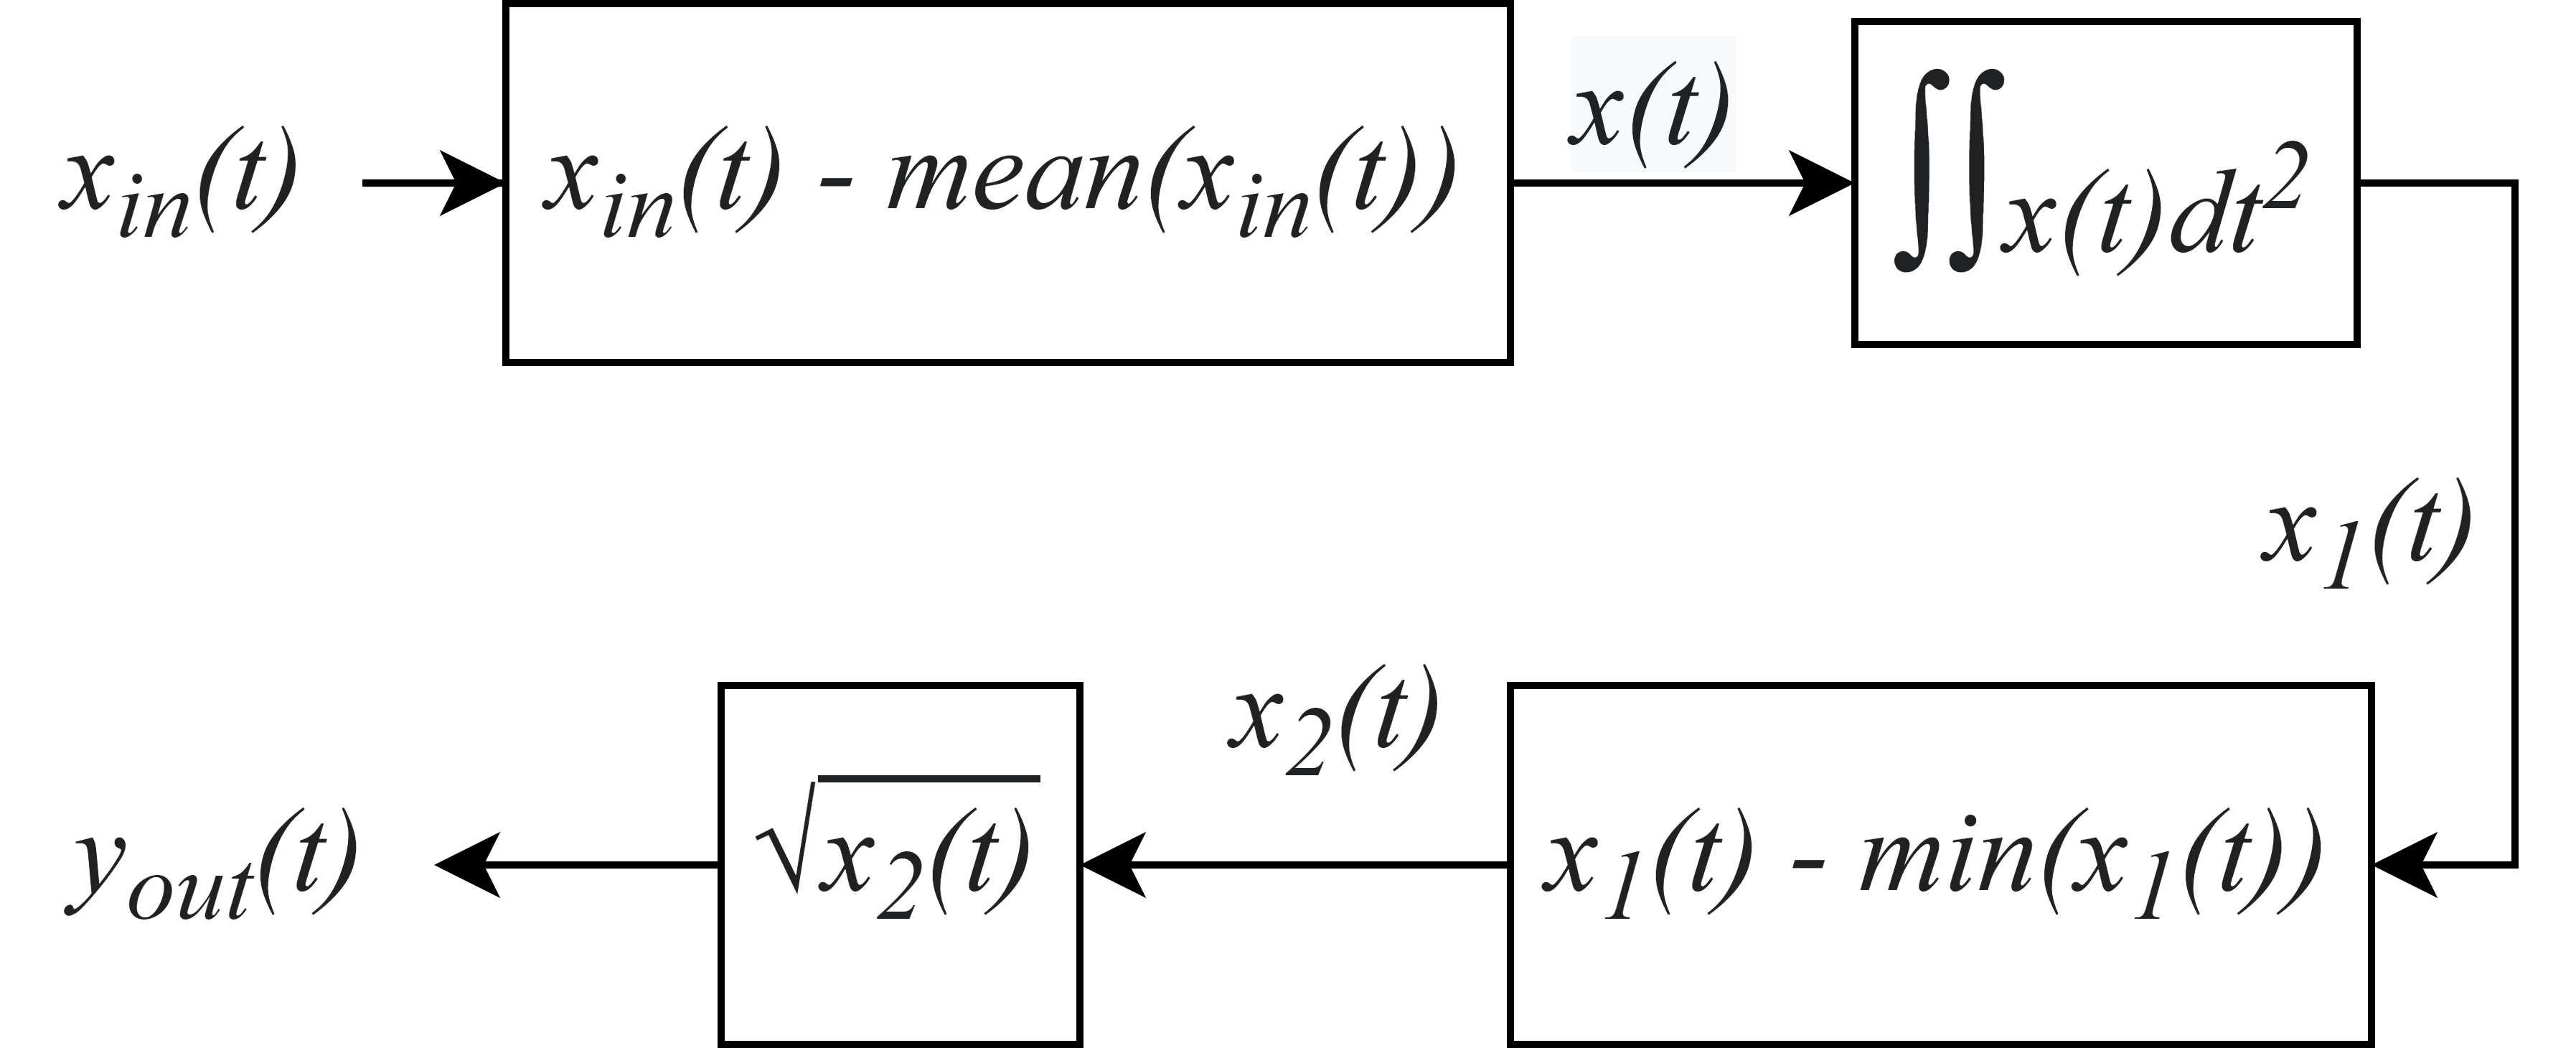
\includegraphics[width=\textwidth]{Figures/Preprocessing Design.png}
    \caption{Signal Pre-processing flowchart}
    \label{fig:sigpreprocessflow}
\end{figure}
\subsection{Proof of concept designs}

To initially experiment with the phenomenon, a small 7 element transducer array was constructed.

\subsection{Amplifier design}

\subsection{Ultrasonic array design}

\subsubsection{Element packing}
To maximise the directivity of the ultrasonic array, the distance between the centroids of all the neighbouring transducers must be minimised. This forms a more densely packed element array and thus, a more uniform beam pattern.
To maximise the density of the transducers, a class of optimization called packing can be used. The aim of packing is to insert geometric shapes in a container as densely as possible.

\begin{figure}[h!]
\centering

    \begin{minipage}{0.4\textwidth}
    \centering
    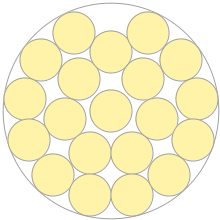
\includegraphics[width= \textwidth]{Figures/Packing/DensestPacking_r0.8_R4.1.png}
    \caption{Densest possible pattern in a circle of radius 4.1cm}
    \label{fig:densest4.1}
    \end{minipage}\hfill
    \begin{minipage}{0.4\textwidth}
    \centering
    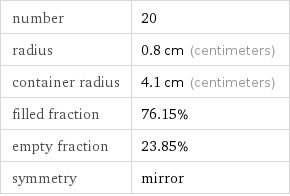
\includegraphics[width= \textwidth]{Figures/Packing/DensestPacking_r0.8_R4.1_packingPercent.png}
    \caption{Densest density information for a circle of radius 4.1cm}
    \label{fig:densest4.1_packinginfo}
    \end{minipage}
    
\end{figure}


\begin{figure}[h!]
\centering

    \begin{minipage}{0.4\textwidth}
    \centering
    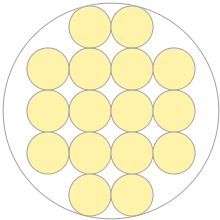
\includegraphics[width= \textwidth]{Figures/Packing/SquarePacking_r0.8_R4.1.png}
    \caption{Square packing pattern in a circle of radius 4.1cm}
    \label{fig:square4.1}
    \end{minipage}\hfill
    \begin{minipage}{0.4\textwidth}
    \centering
    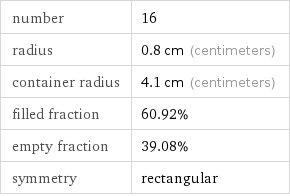
\includegraphics[width= \textwidth]{Figures/Packing/SquarePacking_r0.8_R4.1_packingPercent.png}
    \caption{Density information with square packing for a circle of radius 4.1cm}
    \label{fig:squaret4.1_packinginfo}
    \end{minipage}
    
\end{figure}



\begin{figure}[h!]
\centering

    \begin{minipage}{0.4\textwidth}
    \centering
    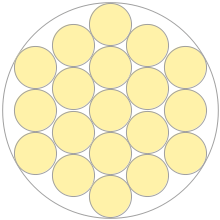
\includegraphics[width= \textwidth]{Figures/Packing/hexagonalPacking_r0.8_R4.1.png}
    \caption{Hexagonal packing pattern in a circle of radius 4.1cm}
    \label{fig:hex4.1}
    \end{minipage}\hfill
    \begin{minipage}{0.4\textwidth}
    \centering
    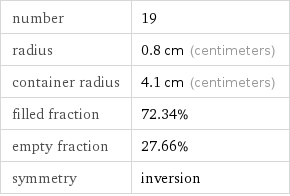
\includegraphics[width= \textwidth]{Figures/Packing/hexagonalPacking_r0.8_R4.1_packingPercent.png}
    \caption{Density information with hexagonal packing for a circle of radius 4.1cm}
    \label{fig:hex4.1_packinginfo}
    \end{minipage}
    
\end{figure}



\begin{figure}[h!]
\centering

    \begin{minipage}{0.4\textwidth}
    \centering
    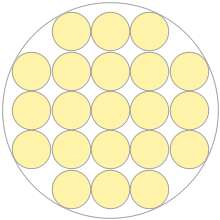
\includegraphics[width= \textwidth]{Figures/Packing/SquarePacking_r0.8_R4.5.png}
    \caption{Square packing pattern in a circle of radius 4.5cm}
    \label{fig:sqr4.5}
    \end{minipage}\hfill
    \begin{minipage}{0.4\textwidth}
    \centering
    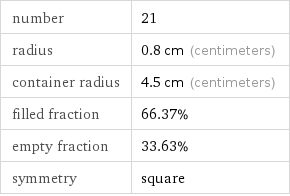
\includegraphics[width= \textwidth]{Figures/Packing/SquarePacking_r0.8_R4.5_packingPercent.png}
    \caption{Density information with square packing for a circle of radius 4.5cm}
    \label{fig:sqr4.5_packinginfo}
    \end{minipage}
    
\end{figure}

%commented this out because it doesn't serve much purpose
\begin{comment}
\begin{figure}[h]
\centering

    \begin{minipage}{0.4\textwidth}
    \centering
    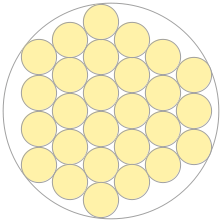
\includegraphics[width= \textwidth]{Figures/Packing/hexagonalPacking_r0.8_R4.9.png}
    \caption{Hexagonal packing pattern in a circle of radius 4.9cm}
    \label{fig:hex4.9}
    \end{minipage}\hfill
    \begin{minipage}{0.4\textwidth}
    \centering
    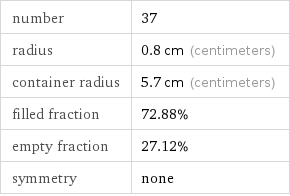
\includegraphics[width= \textwidth]{Figures/Packing/hexagonalPacking_r0.8_R4.9_packingPercent.png}
    \caption{Density information with hexagonal packing for a circle of radius 4.9cm}
    \label{fig:hex4.9_packinginfo}
    \end{minipage}
    
\end{figure}

\end{comment}

\newpage
\subsubsection{Array design simulations}
The purpose of creating the ultrasonic array is to maximise the directivity of the speaker system. To aid in choosing an appropriate array packing profile, some designs were simulated to illustrate the effect that transducer placement has on the radiated beam shape with the goal or reducing side lobes while maximising the main lobe.\\
The transducer patterns from figure \ref{fig:hex4.1} with hexagonal packing and figure \ref{fig:sqr4.5} with square packing were simulated and compared as their designs have symmetry which is required for a uniform beam pattern.\\
To start, a single transducer is modeled and its approximate beam shape simulated with use of a two-dimensional Fourier Transform.
\newpage
\begin{figure}[h!]
\centering

    \begin{minipage}{0.4\textwidth}
    \centering
    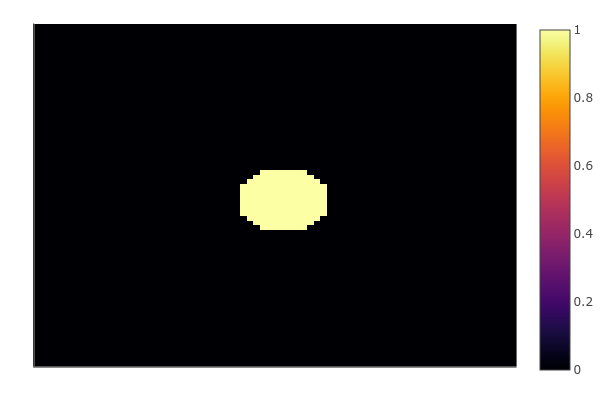
\includegraphics[width= \textwidth]{Figures/arraySim/single/element1.png}
    \caption{Single ultrasonic transducer element to be modeled}
    \label{fig:single_elem}
    \end{minipage}\hfill
    \begin{minipage}{0.4\textwidth}
    \centering
    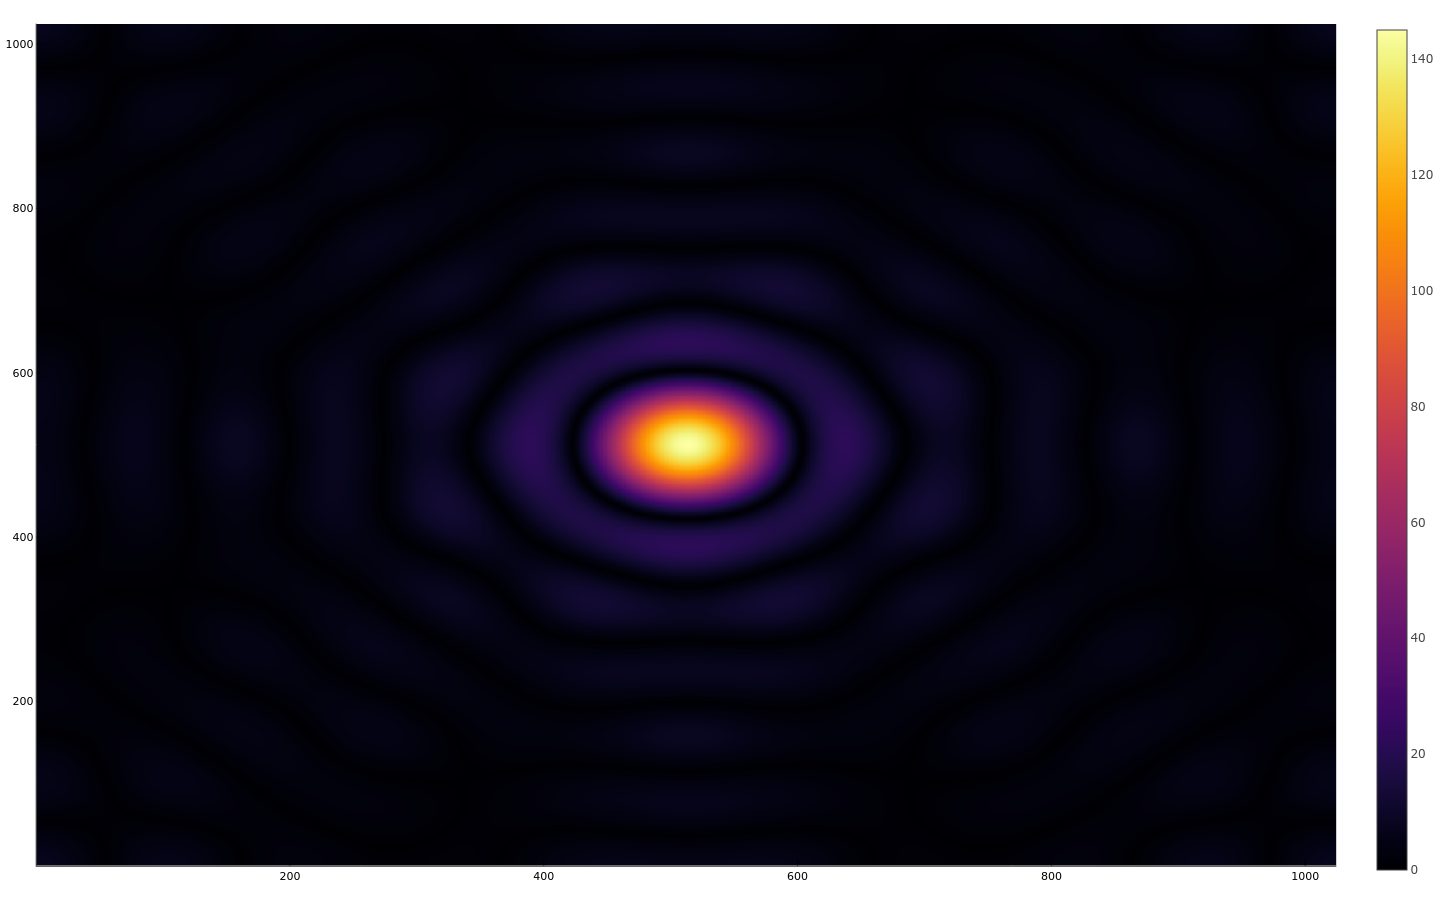
\includegraphics[width= \textwidth]{Figures/arraySim/single/beampat_top.png}
    \caption{Approximate beam shape of a single ultrasonic transducer (Bore-sight view)}
    \label{fig:single_elem_topBeam}
    \end{minipage}
    
\end{figure}
When viewed in three-dimensions, a single element produces the beam shape shown in figure \ref{fig:single_elem_3Dbeam}.
\begin{figure}[ht!]
    \centering
    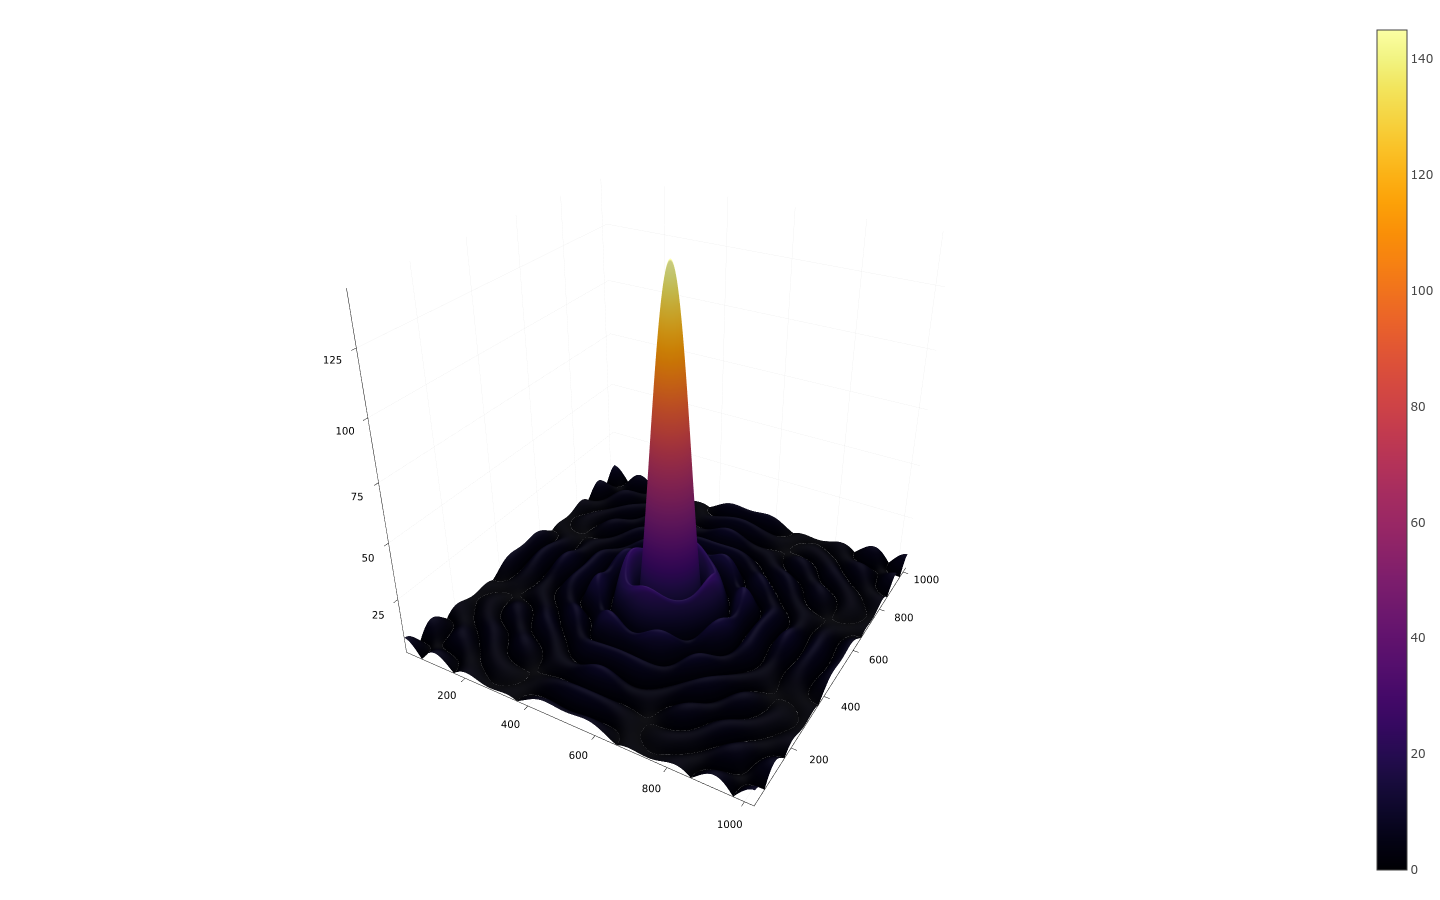
\includegraphics[width=0.8\textwidth]{Figures/arraySim/single/beampat3D.png}
    \caption{Approximate beam shape of a single ultrasonic transducer (3D view)}
    \label{fig:single_elem_3Dbeam}
\end{figure}

Extrapolating the single element into both the hexagonal and square packed designs was done by estimating the spacing between transducers in each design and placing the elements according to this spacing. The square pattern is shown below in figure \ref{fig:sqr_elem} along with its bore-sight beam shape in figure \ref{fig:sqr_elem_topBeam}.
\begin{figure}[h!]
\centering

    \begin{minipage}{0.4\textwidth}
    \centering
    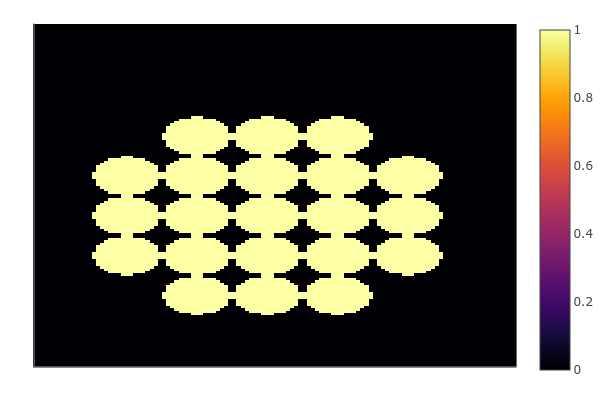
\includegraphics[width= \textwidth]{Figures/arraySim/sqr/arraylayoutcircular.png}
    \caption{Square packed ultrasonic transducer elements to be modeled}
    \label{fig:sqr_elem}
    \end{minipage}\hfill
    \begin{minipage}{0.4\textwidth}
    \centering
    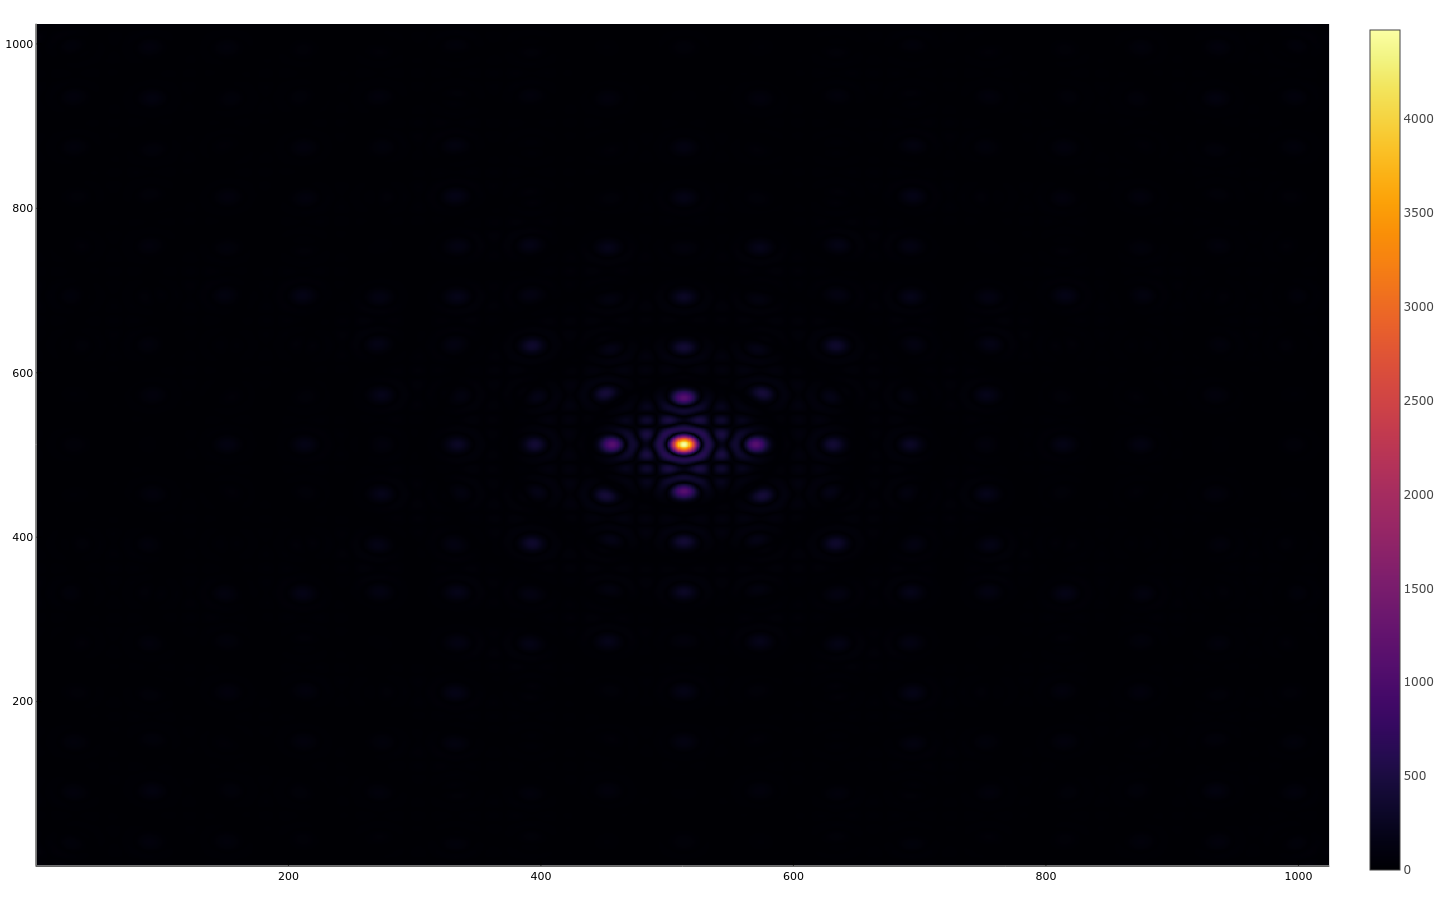
\includegraphics[width= \textwidth]{Figures/arraySim/sqr/circ_sqr_beamTop.png}
    \caption{Approximate beam shape of the square packed ultrasonic transducer array (Bore-sight view)}
    \label{fig:sqr_elem_topBeam}
    \end{minipage}
    
\end{figure}


\begin{figure}[ht!]
    \centering
    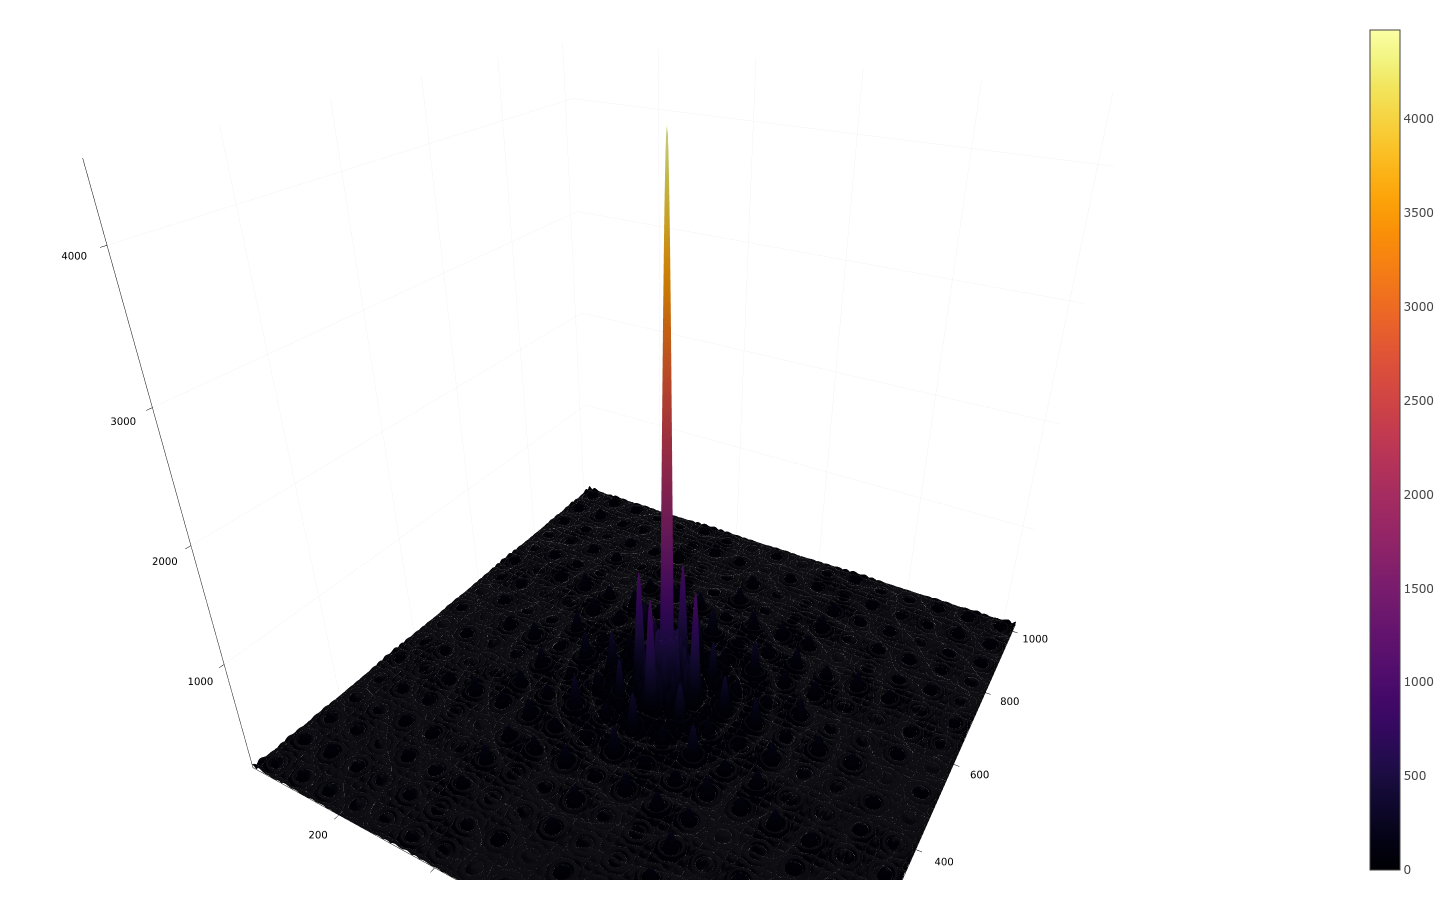
\includegraphics[width=0.8\textwidth]{Figures/arraySim/sqr/circ_sqr_beam3d.png}
    \caption{Approximate beam shape of square packed ultrasonic transducer array (3D view)}
    \label{fig:sqr_elem_3Dbeam}
\end{figure}

The simulation shows that when many evenly spaced transducers are used, it produces a less smooth beam shape due to the discontinuities between elements. For the square packed circular array the beam shape appears to have a significant center lobe with moderately larger side lobes in comparison to the single element simulated in figure \ref{fig:single_elem_3Dbeam}. Since this design has 21 elements, it would produce a larger sound pressure level at its peak than a single element, this proportion should be taken into consideration when deciding on the design.\\

The next simulation aims to reduce the spacing between transducer elements by use of a hexagonal packing as shown in figure \ref{fig:hex4.1}. This design has a filled fraction of 72.34\% which should yield a more uniform beam shape since the discontinuities between transducers have been reduced from the square packed design with a filled fraction of 66.37\% in figure \ref{fig:sqr4.5}. The magnitude of sound pressure energy in this design will be lower than the square design as it only has 19 elements instead of the 21 elements the square packed design contains.\\
The beam shapes were simulated for the hexagonally packed design and are presented in figures \ref{fig:hex_elem} to \ref{fig:hex_elem_3Dbeam}.

\begin{figure}[h!]
\centering

    \begin{minipage}{0.4\textwidth}
    \centering
    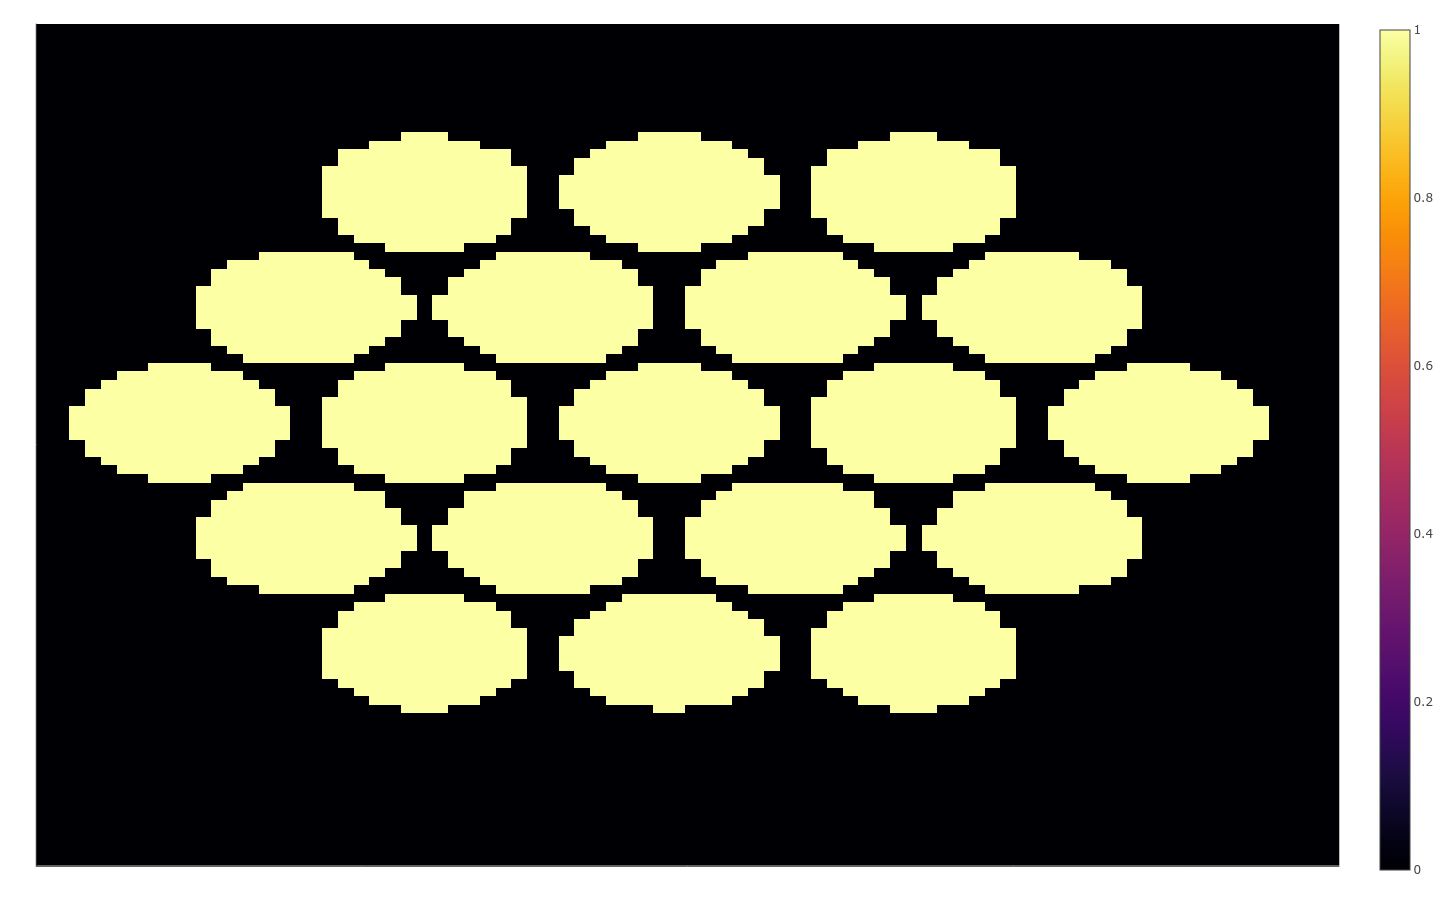
\includegraphics[width= \textwidth]{Figures/arraySim/hex/elemspacing.png}
    \caption{Hexagonally packed ultrasonic transducer elements to be modeled}
    \label{fig:hex_elem}
    \end{minipage}\hfill
    \begin{minipage}{0.4\textwidth}
    \centering
    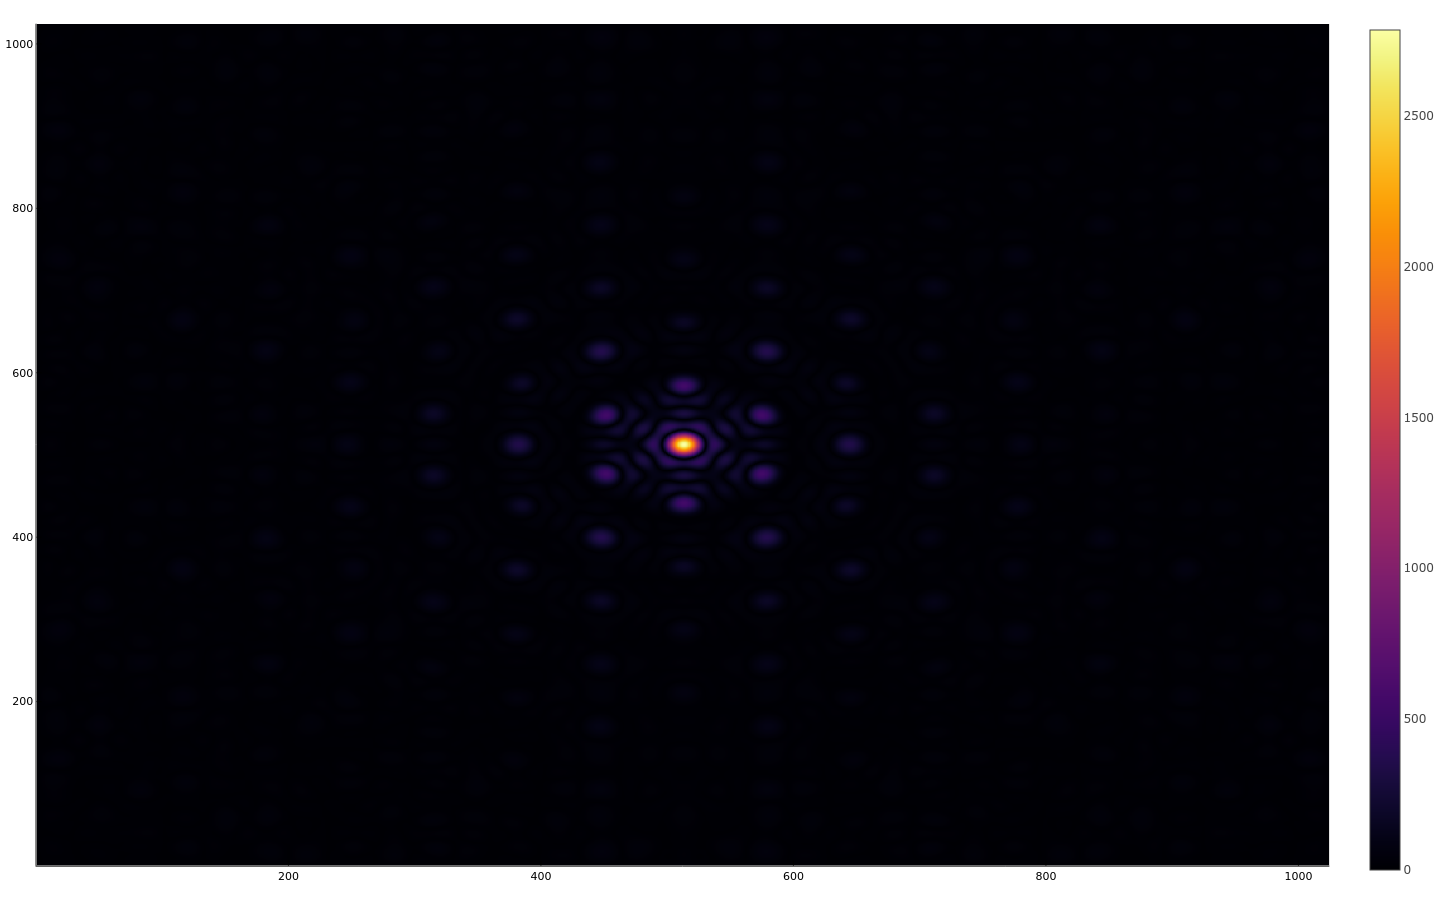
\includegraphics[width= \textwidth]{Figures/arraySim/hex/beampat(top).png}
    \caption{Approximate beam shape of the hexagonally packed ultrasonic transducer array (Bore-sight view)}
    \label{fig:hex_elem_topBeam}
    \end{minipage}
    
\end{figure}


\begin{figure}[ht!]
    \centering
    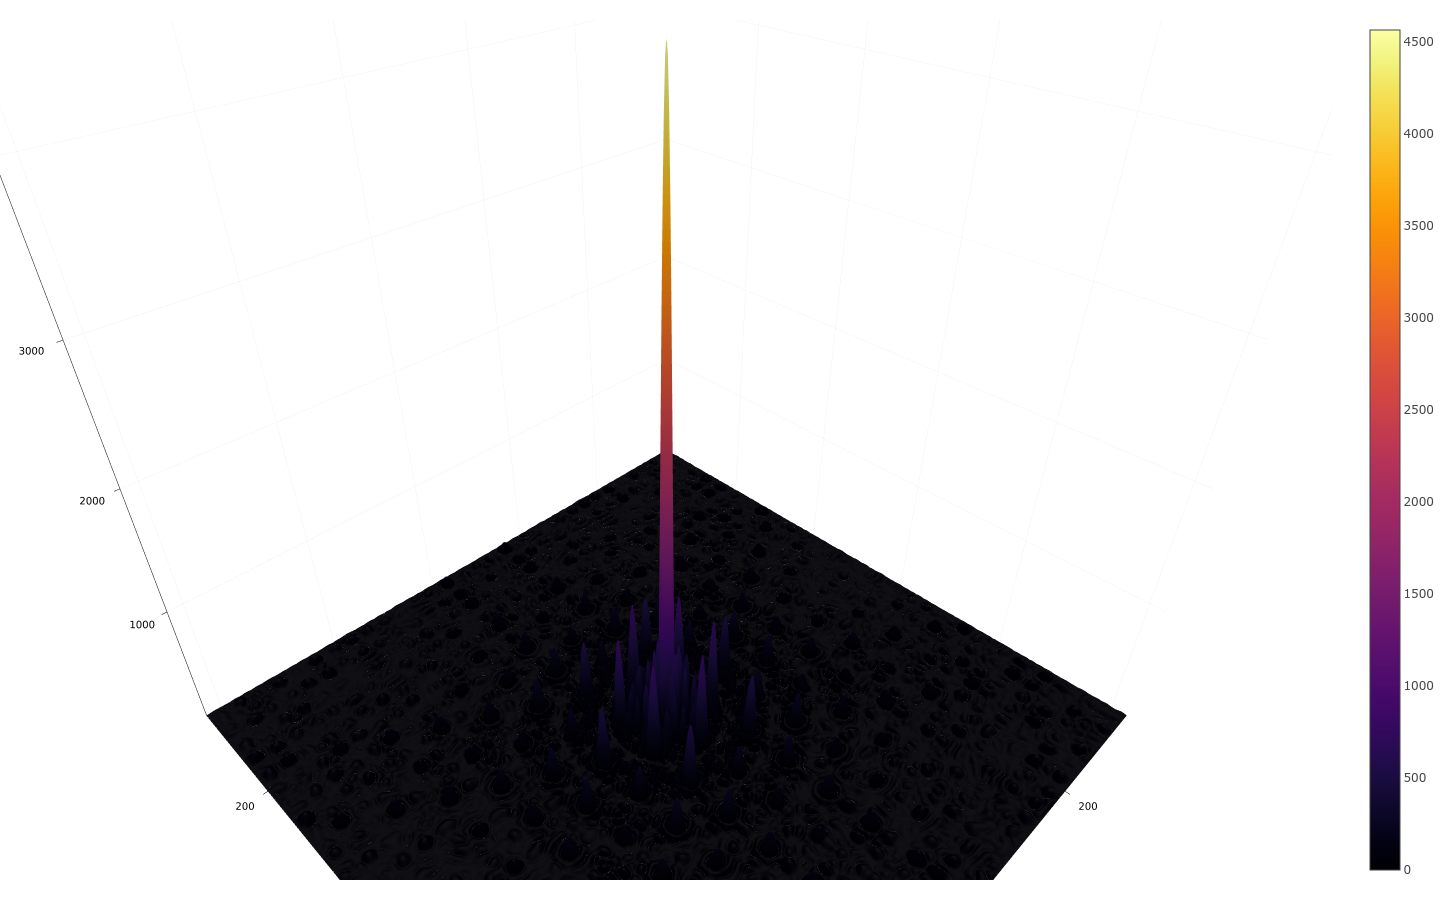
\includegraphics[width=0.8\textwidth]{Figures/arraySim/hex/beampat3dplaneview.png}
    \caption{Approximate beam shape of hexagonally packed ultrasonic transducer array (3D view) with scale}
    \label{fig:hex_elem_3Dbeamscale}
\end{figure}

\begin{figure}[ht!]
    \centering
    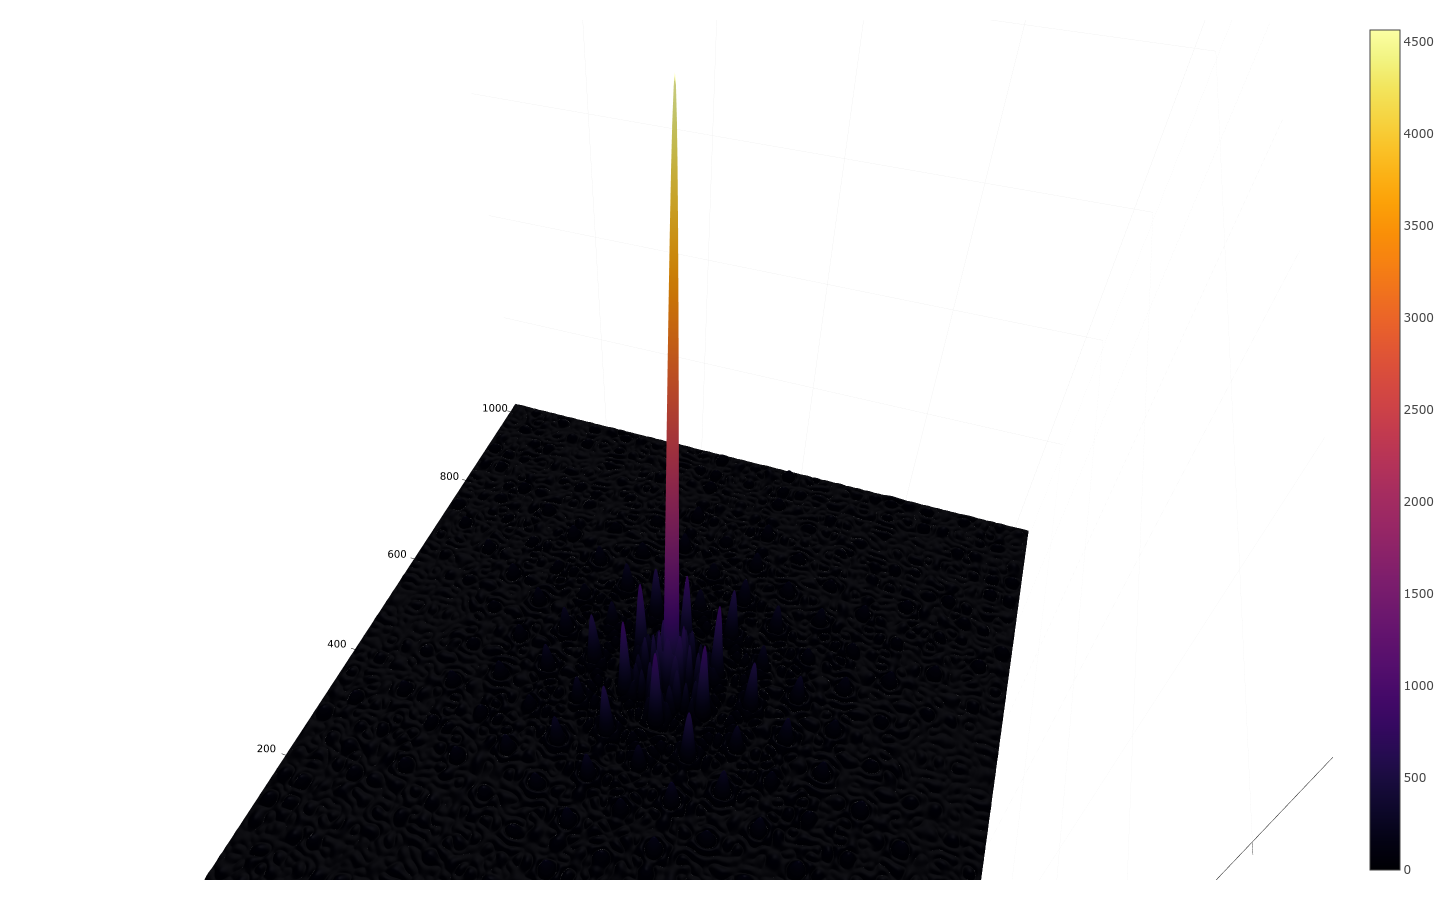
\includegraphics[width=0.8\textwidth]{Figures/arraySim/hex/beampat3d.png}
    \caption{Approximate beam shape of hexagonally packed ultrasonic transducer array (3D shifted view)}
    \label{fig:hex_elem_3Dbeam}
\end{figure}

It can be seen that more side lobes appear when using the hexagonal design, however it does better approximate a single transducer's beam shape with the relatively small lobes surrounding the large main lobe.
\subsubsection{Array PCB design}

